\yesmargins

\chapter{Code Smells and Refactoring}

\begin{tikzpicture}[overlay,remember picture] 
\node[anchor=south] at ([yshift=5in,xshift=0.85in]current page text area.south){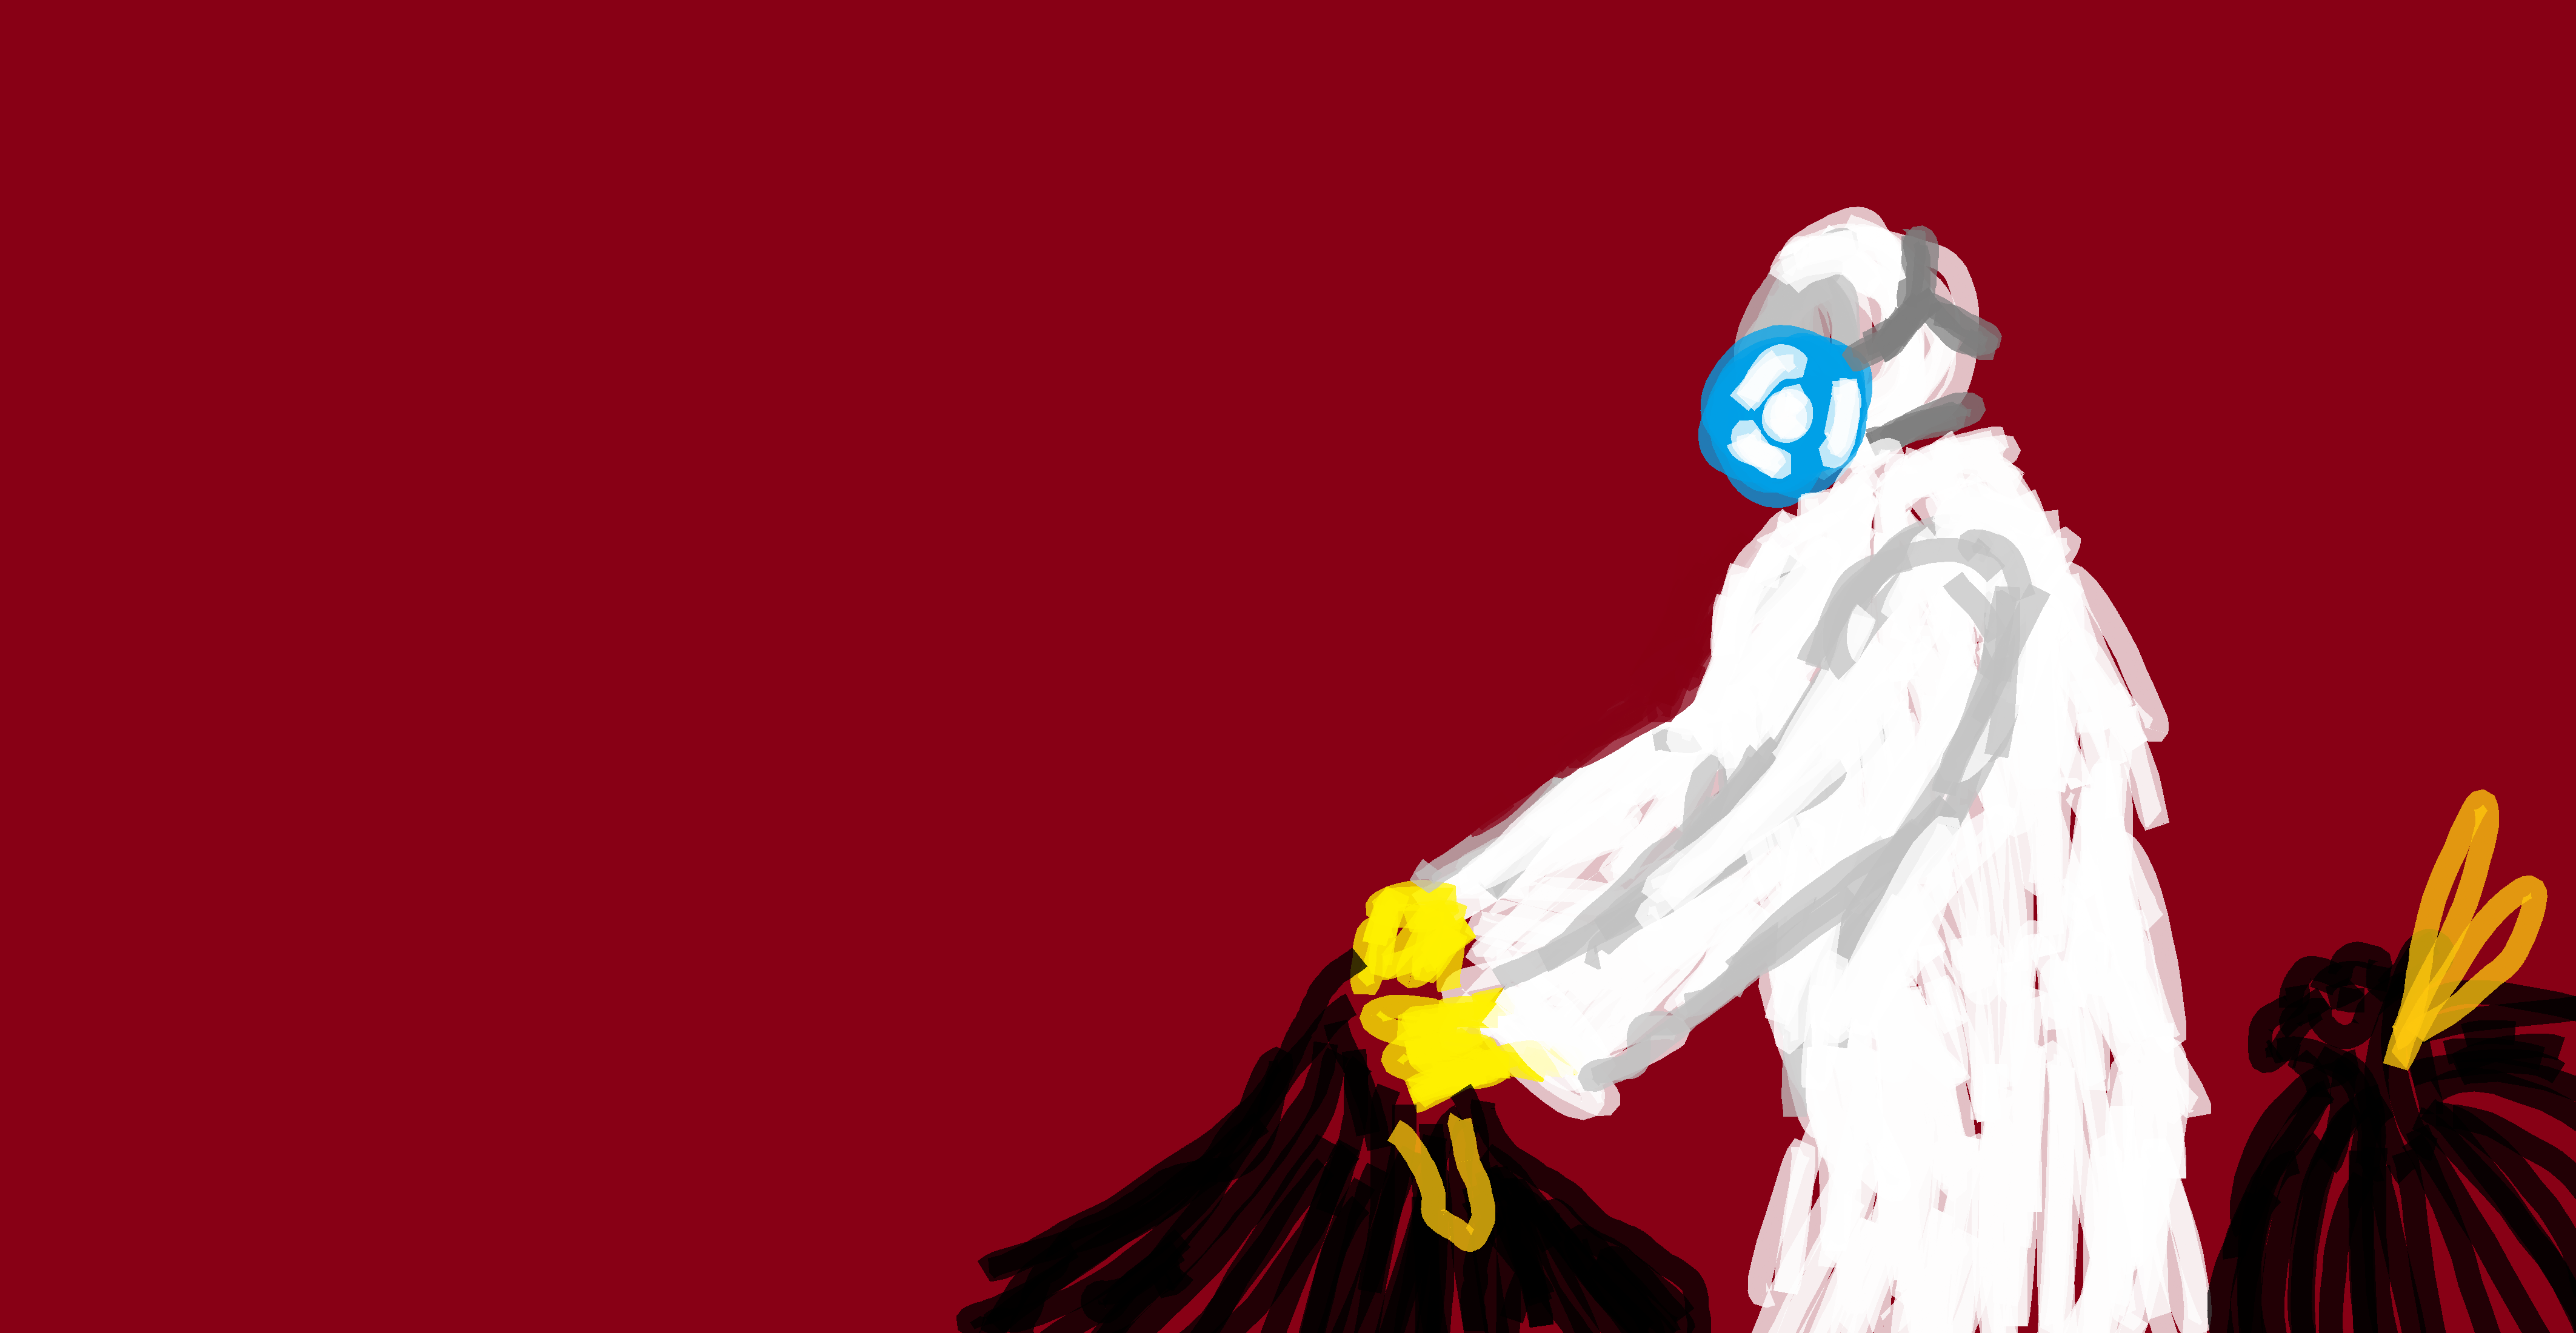
\includegraphics[width=9in]{smells01}}; 
\end{tikzpicture} 

\textbf{Code smells}\index{code smells} are aspects of code that indicate the code needs to be reorganized---signs your software is \textbf{decaying}\marginpar{\codeSmellDef\margindivider}\marginpar{\codeDecayDef}. Your code might need attention if you're having thoughts like these:

\begin{itemize}
\item ``I would \textbf{never show this code} during an interview.''
\item ``I'm going to \textbf{start over} and re-write this code from scratch.''
\item ``Every time I look at this code, I have to \textbf{re-figure-out} what it does.''
\item ``I \textbf{don't} think these code comments \textbf{match} what the code is doing...''
\item ``Why is this code is \textbf{repeated} in three different places?''
\item ``I want to switch out this component, but \textbf{that'll break} X, Y, and Z in this other place and I don't want to deal with that.''
\end{itemize}

Types of codes smells we'll cover (including how to fix them):\\

\begin{itemize}
\item Code smells about \textbf{comments}
\item Code smells about \textbf{functions}
\item \textbf{General code} smells (e.g., about the code within functions)\\
\end{itemize}

\marginpar{If you want to learn more about any of the code smells and refactorings\index{refactoring} described in this chapter, or want to know MORE ways your code can smell, \parencite{martin13} and \parencite{shvets21} are two good resources.}

\section{Why care about code smells?}\index{code smells}

\textbf{Reasons} to pay attention to and fix code smells:\\

\begin{itemize}
\item Smelly code can be \textbf{harder for you and others to maintain} because the code is unclear. When code is hard to maintain, developers tend to work around it or re-create the same functionality elsewhere.\\
\item Smelly code \textbf{leads to smellier code}. When you let your code become disorganized, you are giving yourself and others the message that smelly code is acceptable. Disorganized code also tends to give us an excuse to be lazy coders. A web development example: If you've used CSS, you may have encountered frustrating situations where the style you're trying to apply is not working---somewhere in the code (e.g., other CSS, HTML, or JS), your style is being overridden. Instead of tracking down the competing code or markup, you use the ``!important'' property which forces the style to be applied. The codebase is a mess anyway, so who cares? Your future self.\marginpar{If you think it's more fun to write code than organize code, you may need to be strict with yourself about using good programming practices.}\\
\item Smelly code builds up \textbf{technical debt}\index{technical debt}. If the code is working, there's never a reason to change it, right? Wrong. Each time you write sloppy code, you are contributing to your project's technical debt. Maybe it works now but, as sloppy software grows, it will get more difficult to deal with. That can mean your company needing to hire more developers to keep productivity up. Instead, productivity can go down because now the old developers are struggling to teach the new developers and everyone is continuing to write sloppy code. Ultimately, the software may have to be redeveloped entirely (which doesn't always solve the problem). Or, the project could fail.
\end{itemize}

\section{Your code stinks, now what?}

If you're in a position to (e.g., your manager allows it), strongly consider \textbf{refactoring}. Refactoring\index{refactoring} is when you improve your code without changing what the code does. Refactoring is how you fight against technical debt\index{technical debt}.\marginpar{\refactoringDef\margindivider}\marginpar{\technicalDebtDef}

The remainder of this chapter is about code smells and how to clean them up. This is not an exhaustive list. You can find a lot more by looking through the resources listed at the end of this chapter.

\section{Comments}

When we first learned to code, many of us didn't write comments: solving problems is fun and coding can be addictive, no time for boring comments! Then, we got more experience, started coding with others, were formally trained on coding, or attempted to pick up an old project, and we saw why comments are useful---and then some of us jumped to the other extreme: too many comments. We explained functions with paragraphs of prose, or even commented each line. It's tedious, but it's the right thing to do, right? Unfortunately (and fortunately), \textbf{too many comments can be as bad as none}.

\subsection{Drawbacks of Having Many Comments}\marginpar{Don't fall into the trap of adding excessive comments to your code before an interview! Some prospective employers specifically look for over-commented code (or can't help but see it) as a indicator of poor programming habits.}

\begin{itemize}
\item {Comments \textbf{get out of date quickly}. If we update the code, then procrastinate on the comments, what we leave can be misleading (to others and our future selves). Also, more comments means greater likelihood some will be neglected, giving us the smelly situation of some accurate and some inaccurate comments. In that case, why would we trust \textit{any} of the comments?\\}
\item{Writing comments for straightforward code \textbf{can distract from the important comments}. If the code was difficult to write, is long, is unique, is complex, or has a ``gotcha'', that code is more important to call attention to with comments.\\}
\item{Writing lots of comments could \textbf{indicate the code needs to be simplified}. Ideally, most of the the code you write will be self-explanatory so that comments are infrequently needed.}
\end{itemize}

\subsection{Code Smells about Comments}\marginpar{As a challenge to myself, I kept the code example boxes narrow and tried to make the ``good'' code fit.}

Below is a concise \textbf{list of common code smells}\index{code smells} about comments and what to do about them (how to refactor).\\

\begin{itemize}
\item {
\textbf{Obsolete Comment} (no longer describes the code).\\
Remove or update.
\lstinputlisting[language=Python]{code/csr-comments-obsolete.py}\spacer
}
\item {
\textbf{Commented-Out Code} (somebody thought they'd need that code later, but the commented out block is now getting out of date and in the way).\\
Remove. If you're feeling risk-averse, save a backup or use a version-control system.\marginpar{Commenting out code often comes with poor assumptions (e.g., you'll need the code later, others will understand why you commented it out, the surrounding code will continue having the same purpose, etc.)}
\lstinputlisting[language=Python]{code/csr-comments-deadcode.py}\spacer
}
\item {
\textbf{Redundant Comment} (states what would already be immediately apparent to a programmer of any level).\\
Remove. Less is more.
\lstinputlisting[language=Python]{code/csr-comments-redundant.py}\spacer
}
\item {
\textbf{Long Comment} (multiple sentences, complicated, goes into a lot of detail)\\
Simplify the code to make it more self-explanatory, shorten or remove comment.
\lstinputlisting[language=Python]{code/csr-comments-long.py}\spacer
}
\end{itemize}

\section{Functions}

\marginpar{If you're only writing a short program, does coding style matter? Treating code as disposable is a self-fulfilling prophecy.}A natural way to code is to start writing a function and then, as the program gets more complicated, keep adding to it. For example, if your program's GUI only has a start and a stop button, the function for populating the screen with UI elements need only draw those two buttons. Then, when you add a menu and a settings button, you could update the function to draw those elements, too. Then you add user accounts and decide that function is a fine place to check if the user is logged in, their level of inactivity, show a pop-up about cool new features... and your function balloons. Understanding the small details of how the function works can even make one feel proud---until the \textbf{code becomes unmaintainable and bug-ridden}.  

\subsection{Code Smells about Functions}

\marginpar{Software made of 3 to 4-line functions is amazing to behold!}Follow these \textbf{refactoring suggestions} to increase code readability, maintainability, and modularity.\\

\begin{itemize}

\item{\textbf{Long Function} (more than 10 lines or so)\\Break into multiple functions. Aim for five lines or fewer.\\}

\item{\textbf{Function with Many Jobs} (doing more than what its name suggests, doing things that aren't closely related, doing many things)\\
Break into multiple functions.
\lstinputlisting[language=Python]{code/csr-functions-manyjobs.py}\spacer} 
\item{\textbf{Function with Many Parameters} (more than four, some say more than three)\\
\marginpar{Zero function parameters is even better than four!}As appropriate, pass an object that combines the parameters, make calls within the function to get the parameter data, break into multiple functions, or find another way of reducing the number of parameters.
\lstinputlisting[language=Python]{code/csr-functions-manyparams.py}\spacer}

\end{itemize}

\section{Code}

\marginpar{Code smells\index{code smells} should not be refactored blindly. Always consider how your changes might affect the rest of your software; living with smells is sometimes the wiser choice.}Code \textbf{gets messy fast} if you're not paying attention. One reason is because many of us weren't trained to be neat with code when we first learned it. To write tidy code, you may have to frequently \textbf{stop and think} about its design, or be strict with yourself about \textbf{refactoring regularly}. Over time, you might adopt better habits.

\subsection{Code Smells about Code in General}\index{code smells}

\begin{itemize}
\item{\textbf{Duplicate Code} (same code in multiple places)\\Consolidate into one place, but watch out for creating unwanted dependencies.
\lstinputlisting[language=Python]{code/csr-code-duplicate.py}\spacer}
\item{\marginpar{Thresholds like ``100 characters'' or ``5 lines'' are somewhat arbitrary. Generally, shorter is better, but not even that rule can be applied everywhere. For example, \textit{syntactic sugar} is the term for concise and elegant code syntax, usually built into the programming language. It can make your code shorter, but what's the point if nobody can understand it!}\textbf{Long Lines} (more than 100 characters or so)\\Shorten by breaking into multiple lines, converting to a function call, defining new variables, etc.
\lstinputlisting[language=Python]{code/csr-code-longline.py}\spacer}
\item{\textbf{Inconsistent Conventions} (formatting code differently in different places, or untidily)\\Follow whatever style conventions the code is already using. If it's a new project, plan to be self-consistent or follow accepted conventions for the language you're using.\marginpar{When adding to another person's code, it's best to follow their coding style conventions even if you prefer a different way. However, if their code style is sloppy and inconsistent, consider whether there's a polite way to fix the problem.}
\lstinputlisting[language=Python]{code/csr-code-consistent.py}\spacer}
\item{\textbf{Vague Naming} (does not communicate what the function, variable, etc. is for)\\Rename it, even if the name is long. Long names can sometimes replace comments.\marginpar{Wouldn't it be nice if code read like a book?}
\lstinputlisting[language=Python]{code/csr-code-descriptive.py}\spacer
}
\end{itemize}

\nomargins
\section{Conclusion}
Cleaning up your code can help make your software sustainable and extensible and can make your teammates happier too.

\section{Additional Resources}

\begin{description}
\item \fullcite{fowler19}
\item \fullcite{guizani2020gender}
\item \fullcite{martin13}
\item \fullcite{shvets21}
\end{description}